% ----------------------------------------------
% INTRODUCAO
% ----------------------------------------------
\chapter{Introdução}\label{cap:introducao}

A base para o desenvolvimento de um sistema de monitoramento digital capaz de acompanhar produtos perecíveis, passa por um entendimento de todos os elos envolvidos. Dentre eles a dinâmica entre a temperatura e o crescimentos de vida microbiana (Listeria) bem como a logística nacional para esse tipo de alimento. Além disso, deve-se considerar também as limitações técnicas para o desenvolvimento de dispositivos IoT capazes de obter dados críticos de todo o processo.

Neste trabalho pretende-se propor um dispositivo capaz acompanhar o deslocamento de um determinado alimento perecível. Para isso, esse dispositivo, necessita possuir alguns requisitos como:
\begin{itemize}
    \item Baixo valor agregado, uma vez que precisa ser empregado em caixas de transporte de alimentos;
    \item Ocupar a menor área possível;
    \item Operar sem a necessidade trocas de pilhas ou recarregamento de baterias;
\end{itemize}

A definição destes requisitos, passa também por um entendimento das condições de operação e ambiente a que esse sistema está submetido, bem como os agentes envolvidos para um correto entendimento do cenário completo.
%%%%%%%%%%%%%%%%%%%%%%%%%%%%%%%%%%%%%%%%%%%%%%%%%%%%%%%%%%%%%%%%%%%%%%
\section{Produtos perecíveis}
%%%%%%%%%%%%%%%%%%%%%%%%%%%%%%%%%%%%%%%%%%%%%%%%%%%%%%%%%%%%%%%%%%%%%%
Denominam-se alimentos perecíveis aqueles que possuem uma quantidade significativa de água. Isso os torna vulneráveis a proliferação de vida microbiana que é a principal responsável pela decomposição destes alimentos. Para se manterem conservados, estes alimentos necessitam manter-se refrigerados.
Alimentos perecíveis estão presentes no dia a dia das populações no mundo inteiro, pois muitos deles são a base de uma alimentação saudável devido a pouca exposição a conservantes ou processos industriais que embora eliminem as suas bactérias, acabam por eliminar também os seus nutrientes.
Com o objetivo de mapear a composição dos principais alimentos consumidos no Brasil, a \citeonline{Anvisa2011} desenvolveu o projeto TACO (Tabela Brasileira de Composição de Alimentos). A partir desta, obteve-se um detalhamento da tabela nutricional e demais dados dos alimentos que compõe o dia a dia dos brasileiros.

Com base nisso, apresenta-se um problema relacionado a distribuição destes alimentos ao longo de um país como o Brasil que possui dimensões continentais e alguns alimentos são produzidos apenas em certas regiões.
Com o objetivo de predizer o impacto do aumento de listeria \citeonline{monica} apresenta um algorítimo baseado em redes neurais artificiais \textit{Multilayer Perceptron} (MLP) em função dos impactos atmosféricos a que esses alimentos são submetidos. A capacidade de prever a vida útil destes alimentos a partir de fatores ambientais pode ser decisivo para a escolha do meio de transporte do mesmo e para o aumento das exigências de qualidade que redes atacadistas impõe no ato de revenda dos mesmos.

%%%%%%%%%%%%%%%%%%%%%%%%%%%%%%%%%%%%%%%%%%%%%%%%%%%%%%%%%%%%%%%%%%%%%%
\section{Logística}
%%%%%%%%%%%%%%%%%%%%%%%%%%%%%%%%%%%%%%%%%%%%%%%%%%%%%%%%%%%%%%%%%%%%%%
Dentro de uma cadeia de distribuição de alimentos, existe uma série de desafios logísticos envolvidos no processo e todos esses processos são responsáveis por um grau de depreciação na vida útil de alimentos como frutas, verduras e legumes (FLV). Analisar essa cadeia é essencial para compreender que quanto mais elementos envolvidos, como intermediários, maior as chances de se perder a rastreabilidade e a qualidade dos FLV.
Os autores \citeonline{Aliotte2022} detalham que os fatores mais importantes a serem observados no processo de distribuição são:
\begin{itemize}
    \item Tipo de transporte
    \item Agente responsável pelo transporte
    \item Rastreabilidade
    \item Acondicionamento em câmara fria
    \item Tipos de embalagem
    \item Troca de embalagem
    \item Manipulação da carga
\end{itemize}

Dentre estes, cabe destaque para o tipo de transporte, que pode ser do tipo caminhão baú frigorificado que pode oferecer temperaturas abaixo de $0^oC$; caminhão baú refrigerado que pode manter temperaturas entre $0^oC$ e $12^oC$; caminhão graneleiro que possui apenas proteção com lona para orvalho, sol e chuva e não possui controle de refrigeração; caminhão baú sem refrigeração que se assemelha ao graneleiro; além do caminhão com carroceria aberta. Na figura~\ref{fig:transporte} é possível ver a distribuição de uso destes caminhões para alguns tipos de cargas.

\begin{figure}
  \caption{Transporte por tipo de carroceria.}
  \begin{center}
      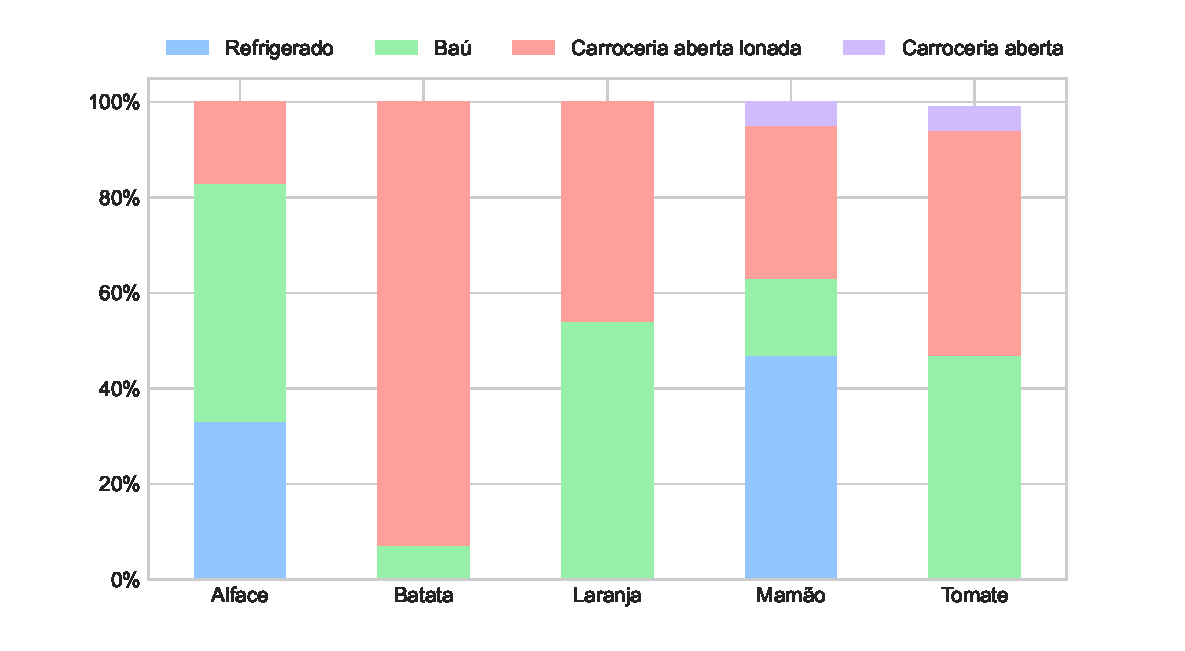
\includegraphics[trim={0 1.2cm 0 0.5cm },scale=0.6]{img/transporte.pdf}
  \end{center}
  \fonte{Elaborado pelo autor com base em~\cite{Aliotte2022} }
  \label{fig:transporte}
\end{figure}

Uma vez introduzidas as diferentes formas de transporte \citeonline{Aliotte2022} discorrem sobre os agentes responsáveis pelo transporte e suas particularidades. Fatores como distância a ser percorrida e a terceirização do transportes são efetivamente relevantes, impactando diretamente na qualidade dos FLV.

Ao tratar da rastreabilidade e acondicionamento em câmara fria, \citeonline{Aliotte2022} apontam uma demanda do mercado por qualidade. Fica evidente que investimentos nessas áreas possuem um apelo não só para atender consumidores exigentes como normas sanitárias.

Já os três últimos tópicos: tipos de embalagem, troca de embalagem e manipulação da carga, dizem respeito aos impactos da embalagem tanto ao condicionamento como ao desgaste ocasionados no processo de alocação.

``Para que o produto chegue ao destino em boas condições, é necessário que ocorra o mínimo de manuseio, que sejam cumpridas as regras sanitárias nas operações de carga e descarga, além do uso de tecnologias que reduzam a manipulação por ação humana.'' \cite[p.~16]{Aliotte2022}





%%%%%%%%%%%%%%%%%%%%%%%%%%%%%%%%%%%%%%%%%%%%%%%%%%%%%%%%%%%%%%%%%%%%%%
\section{IoT}
%%%%%%%%%%%%%%%%%%%%%%%%%%%%%%%%%%%%%%%%%%%%%%%%%%%%%%%%%%%%%%%%%%%%%%
O termo \textit{Internet of Things} (IOT), traduzido livremente para ``Internet das Coisas'', popularizou-se nos últimos anos devido aos avanços tecnológicos em termos de miniaturização de circuitos eletrônicos. Graças a esses avanços, um mundo de opções se abriu para resolver problemas que antes eram impossíveis como o controle de iluminação artificial em uma horta apresentado por \citeonline{9268238} que controla um sistema de espelhos para garantir um adequado fornecimento de luz, além de coletar informações disponibilizando-as em uma plataforma web.

Dispositivos IOT tem como princípio básico o acesso direto a internet, seja para apenas enviar informações, apenas receber ou ambos. A principal vantagem desses sistemas se dá em função da possibilidade de externar o processamento, garantindo assim um requisito de hardware mínimo local, deixando tarefas complexas para a rede externa (Nuvem).  

A popularização dos sistemas IOT se dá de forma tão rápida que até mesmo problemas decorrentes da sincronização de dispositivos passam a ser tratados com soluções como a apresentada por \citeonline{7924944}. Já aplicações que perdem a adesão são rapidamente descontinuadas como a solução da empresa Amazon para comprar sabão de roupas com um botão instalado na maquina de lavar\citeonline{amazon} mostrado na figura~\ref{fig:amazon}.

\begin{figure}
  \caption{Amazon Dash Button.}
  \begin{center}
      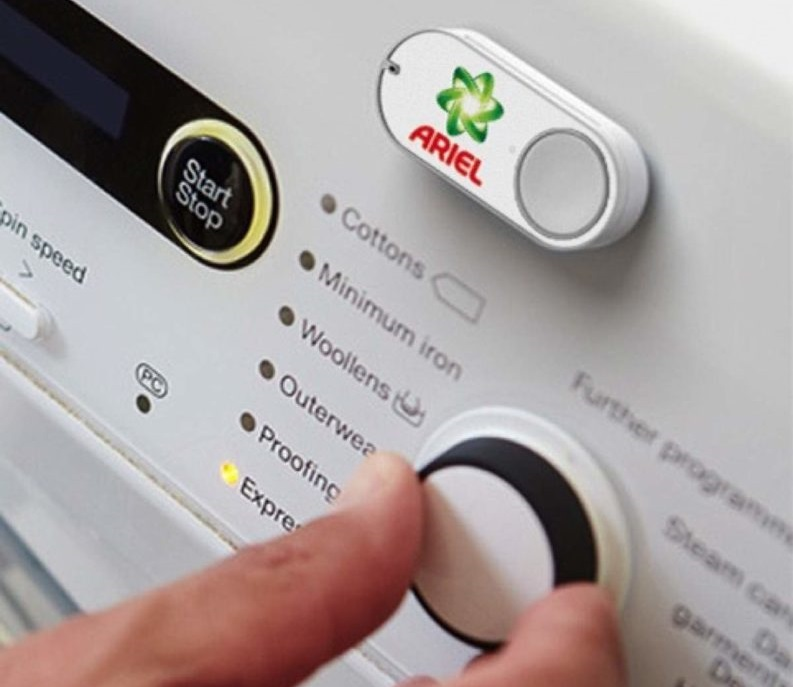
\includegraphics[scale=0.6]{img/Amazon-Dash-Button.png}
  \end{center}
  \fonte{\citeonline{amazondash}}
  \label{fig:amazon}
\end{figure}

Segundo \citeonline{8648462}, os principais desafios para empregabilidade de sistemas IOT são a extrema heterogeneidade que diz respeito aos diferente tipos de dispositivos e protocolos envolvidos, a dinâmica imprevisível que diz respeito aos ambientes distintos e obstáculos físicos além da escalabilidade no núcleo que trata dos problemas que envolvem o acesso de vários dispositivos a uma mesma nuvem. Este último, se apresenta como grande relevância para os próximos anos, pois o aumento da quantidade de ``coisas'' ligadas a internet tendem a crescer em demasia.

%%%%%%%%%%%%%%%%%%%%%%%%%%%%%%%%%%%%%%%%%%%%%%%%%%%%%%%%%%%%%%%%%%%%%%

%%%%%%%%%%%%%%%%%%%%%%%%%%%%%%%%%%%%%%%%%%%%%%%%%%%%%%%%%%%%%%%%%%%%%%








